\newcommand{\erassistant}{ErAssistant~}

\chapter{Построение модели данных}
\label{cha:analysis}
%
% % В начале раздела  можно напомнить его цель
%
В данном разделе описывается процесс создания проекта базы данных в среде \erassistant \textit{(ver. 2.10).}

\section{Работа по методическим указаниям}
Произведем разработку проекта базы данных по теме, утвержденной в рамках дисциплины <<Разработка базы данных>>.
\subsection{Описание предметной области}
Компания занимается производством и продажей небольших статуэток,
раскрашиваемых вручную. Компания имеет несколько производственных
направлений. Миниатюры изготавливаются из гипса, олова или алюминия.

Компания распространяет свои товары по трем каналам. Компания содержит
пять собственных розничных магазинов. Помимо этого, компания владеет
сайтом, на котором ведется online-торговля, и осуществляет оптовые поставки
сторонним
дистрибьюторам.
Для
анализа
статистики,
системой автоматизации производства, нужен интерактивный аналитический
инструмент. Поэтому необходимо спроектировать и построить модель данных,
которая станет хранилищем информации по производству.

В ходе производства изделий система автоматизации производства
управляет всеми станками компании. Каждый станок реализует полный цикл
производства изделий, включая:
\begin{itemize}
	\item заполнение формы сырьем (гипсом, оловом или алюминием);
	\item затвердевание материала;
	\item  удаление изделия из формы после затвердевания;
	\item при необходимости автоматизированная раскраска изделий (оловянные фигурки не раскрашиваются);
	\item сушку после покраски (при необходимости).
\end{itemize}


Покраска и сушка могут производиться за несколько этапов в зависимости
от сложности изделия. По мере готовности изделия проходят проверку,
выполняемую оператором станка.

Оператор станка регистрируется в системе. В ходе этого процесса оператор
сообщает системе автоматизации производства тип производимых изделии и
объем загруженного в машину сырья. Оператор также делает в системе запись
при отбраковке изделий.

В ходе
интервью необходимые для эффективного анализа статистики:
\begin{itemize}
	
	\item  число принятых изделий по объему сырья, видам изделий, машинам и
	\item  время формовки и затвердевания по видам изделий, машинам и дням;
	\item  время покраски и сушки по типам краски, видам изделий, машинам и
	\item  сворачивание по подтипам изделий, которые сворачиваются по типам;
	\item  сворачивание по типам машин, которые сворачиваются по материалам
	(гипс, олово или алюминий);
	\item  сворачивание машин по фабрикам, которые сворачиваются по странам;
	\item  сворачивание дней по месяцам, месяцев — по кварталам;
	\item  возможность фильтрации информации по производителю и дате покупки машины.
\end{itemize}

Анализ файла-экспорта из системы автоматизации производства показал,
что для каждого вида производимых изделий есть отдельная строка, в которой
присутствует следующая информация:
\begin{itemize}
	\item  тип изделия;
	\item  объем сырья;
	\item  номер машины;
	\item  личный номер оператора;
	\item  время и дата начала производства (когда серия начата);
	\item  время и дата окончания производства (когда серия закончена);
	\item  флаг отбраковки.
\end{itemize}
%\newpage
\subsection{Построение модели}
По приведенному описанию предметной области построим ее модель в среде \erassistant. Укажем линии связей, назначим им имена, укажем типы и кратность связей. В результате работы, модель примет вид, приведенный на Рисунке \ref{fig:1-metod}.

% TODO: \usepackage{graphicx} required
\begin{figure}[ht]
	\centering
	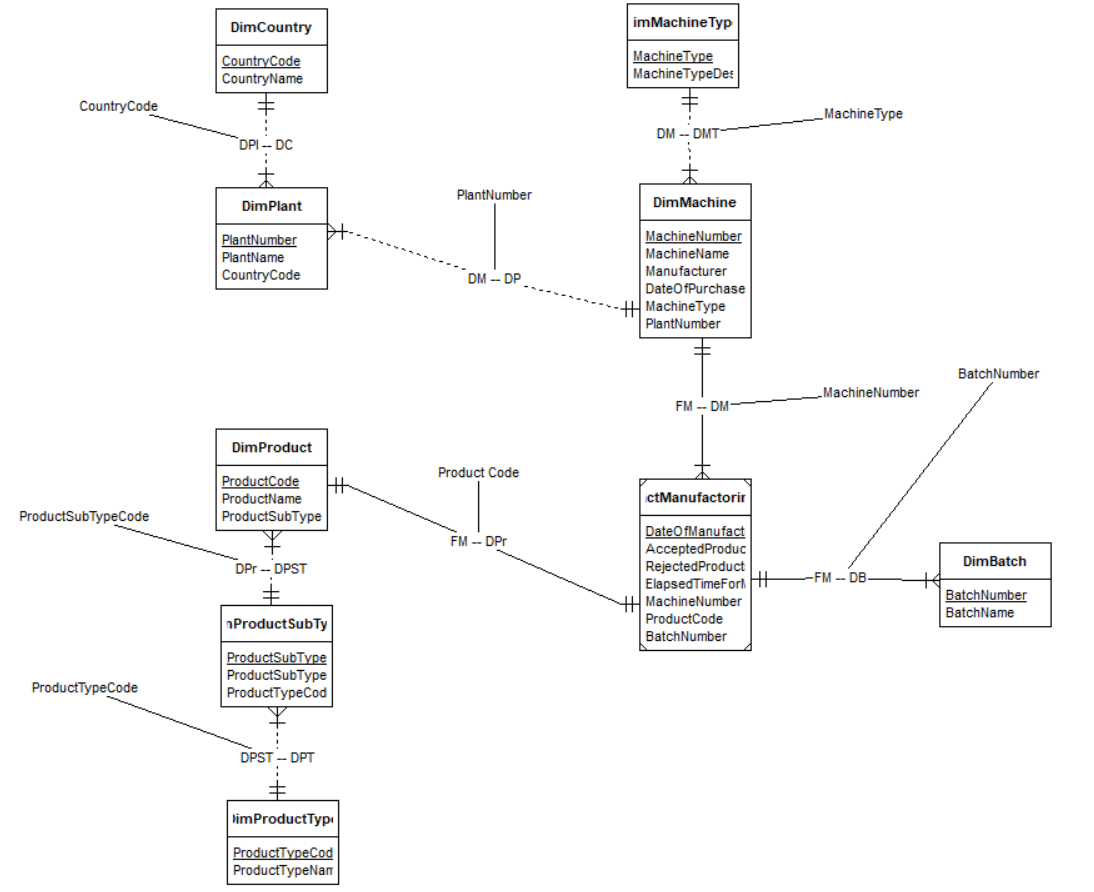
\includegraphics[width=\linewidth]{1-metod}
	\caption{Модель данных Производства со связями}
	\label{fig:1-metod}
\end{figure}
\section{Индивидуальное задание}
Произведем разработку проекта базы данных по индивидуальной теме.
\subsection{Описание предметной области}
В качестве индивидуального задания была выбрана реализация модели информационной системы по хранению и анализу данных  предприятия, занимающегося сборкой и поставкой спортивных велосипедов для конечных потребителей по индивидуальному заказу.

Предприятие располагает широким выборов компонентов и комплектующих для сборки велосипедов следующих типов:
\begin{itemize}
	\item дорожный;
	\item горный;
	\item кросс-кантри;
	\item эндуро;
	\item прогулочный.
\end{itemize}

Предприятие может предложить сконфигурировать велосипед, отдельно выбрав каждый из предложенных компонентов:
\begin{itemize}
	\item рама;
	\item вилка;
	\item руль;
	\item трансмиссия;
	\item колеса;
	\item тормозная система.
\end{itemize}

Контроль над выполнением работ по сборке велосипеда проводится в виде учета всех операций по сборке, настройке и тестированию, проводимых на территории предприятия ее сотрудниками. При этом каждая запись содержит следующую информацию о проведенных работах:
\begin{itemize}
	\item внутренний номер изделия;
	\item время;
	\item этап работ;
	\item название цеха;
	\item имя мастера;
	\item статус;
	\item примечание.
\end{itemize}

На предприятии ведется учет всех компонентов велосипедов.
В базе данных предприятия хранится информация о каждом компоненте, приобретенном у партнеров или изготовленном самостоятельно.

В независимости от типа компонента он обладает общей информацией о наименовании производителя, месте и времени изготовления, типе и рекомендованной розничной цене. 
Также каждый компонент имеет особые сведения, присущие данному типу детали.

\subsection{Построение модели}
После приведения общих сведений о роде деятельности предприятия, факторизируем модель данных информационной системы предприятия в среде \erassistant (cм Рисунок \ref{fig:1-cycle}). Приложение \erassistant позволяет пользователю создавать, редактировать диаграммы сущностей и связей.

Укажем названия связей, их идентификаторы и кратность, исходя из вида отношений, выстроенных между сущностями.
% TODO: \usepackage{graphicx} required
\begin{figure}[h!]
	\centering
	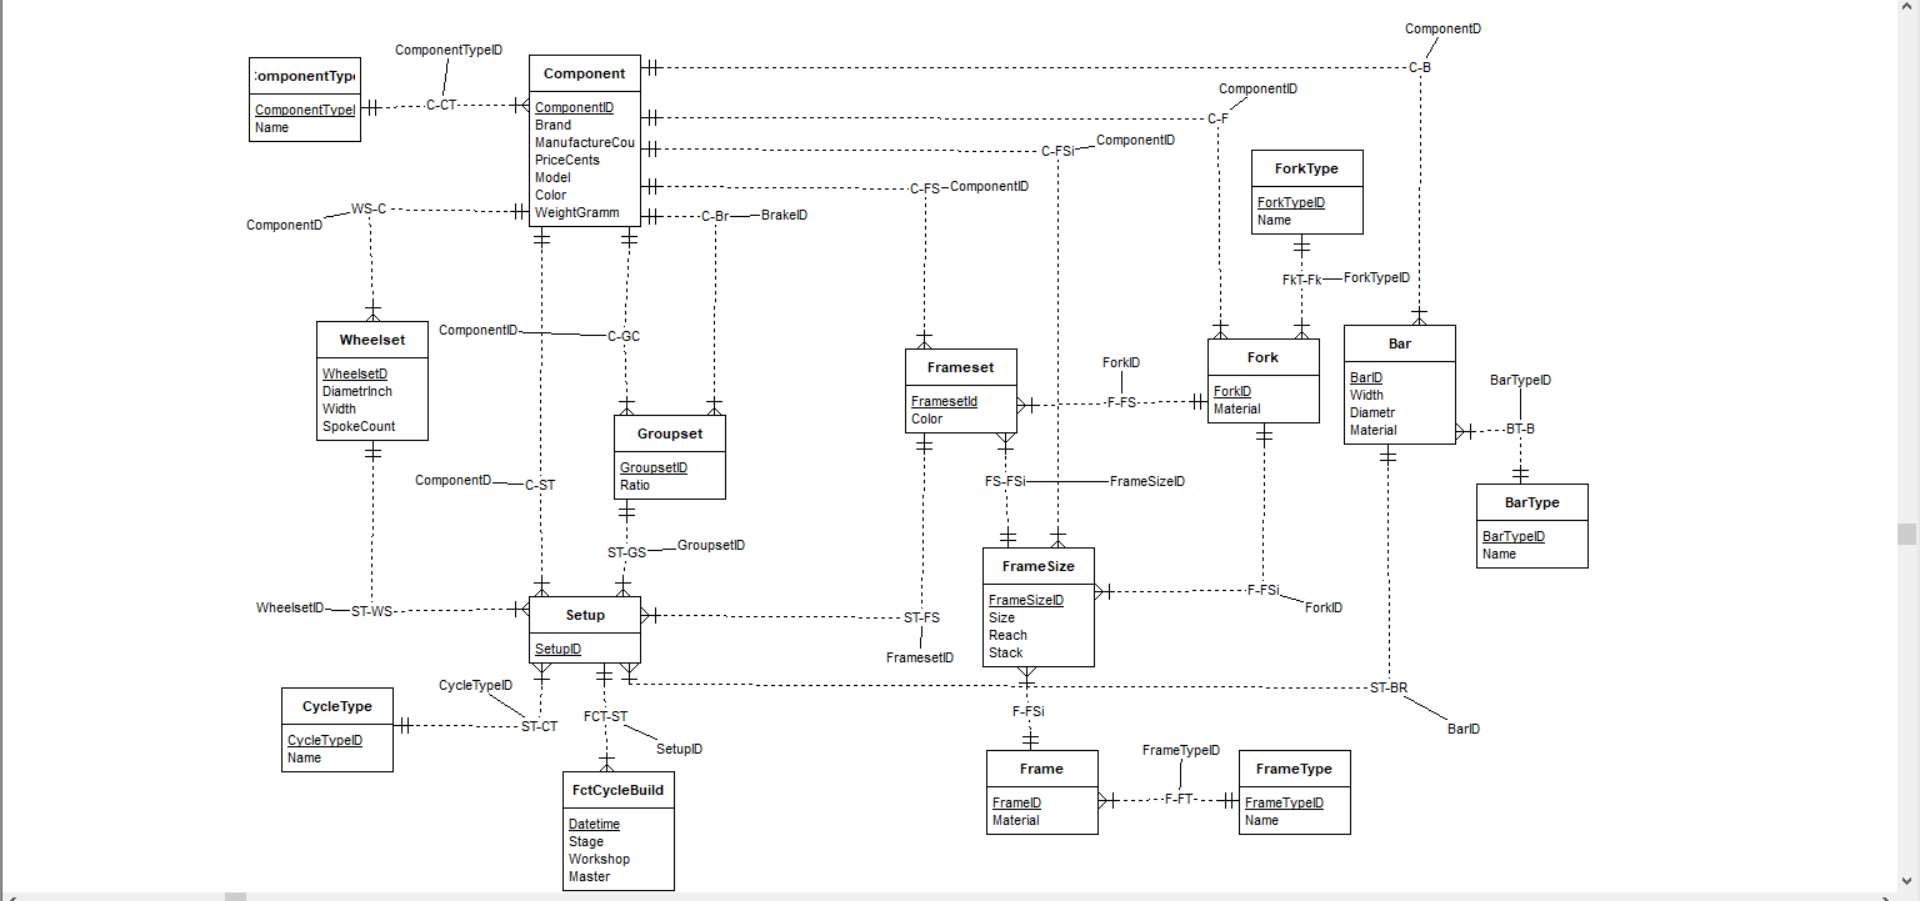
\includegraphics[width=1\linewidth]{1-cycle}
	\caption{Модель данных вело-предприятия}
	\label{fig:1-cycle}
\end{figure}



На данном этапе выполнения работы мы реализовали проект базы данных будущего хранилища данных, планируемого к применению в компании, занимающейся сборкой и поставкой велосипедов по индивидуальному заказу. Был проведен анализ переметной области, определен список сущностей, которые наиболее полно смогут описать сущности, участвующие в производственном процессе.
%%% Local Variables:
%%% mode: latex
%%% TeX-master: "rpz"
%%% End:
